\documentclass{article}
\usepackage{tikz}
\usetikzlibrary{shapes.geometric}

\begin{document}

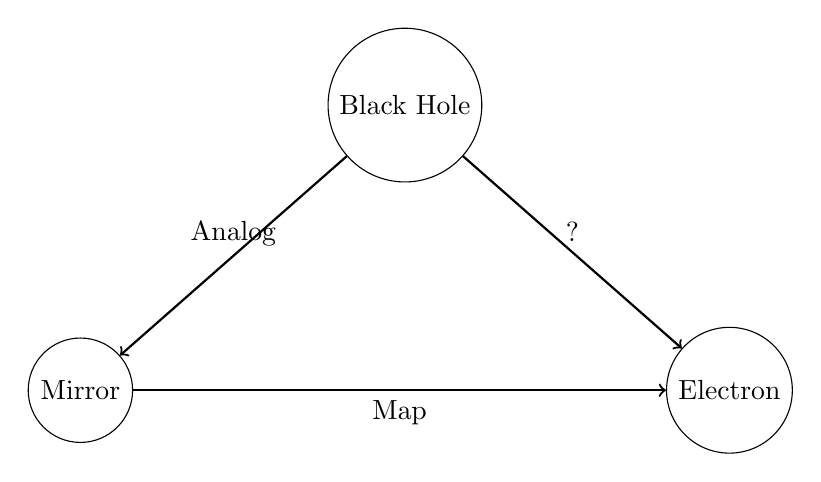
\begin{tikzpicture}[node distance=3cm]
    \node[draw, circle] (black_hole) {Black Hole};
    \node[draw, circle, below left of=black_hole, xshift=-2cm, yshift=-1.5cm] (mirror) {Mirror};
    \node[draw, circle, below right of=black_hole, xshift=2cm, yshift=-1.5cm] (electron) {Electron};

    \draw[->, thick] (black_hole) -- node[midway, above] {Analog} (mirror);
    \draw[->, thick] (black_hole) -- node[midway, above] {?} (electron);
    \draw[->, thick] (mirror) -- node[midway, below] {Map} (electron);

\end{tikzpicture}

\end{document}